
\chapter {Getting Started}

In this chapter we will get started with Oscad. We will run through the various options available on the  with an example circuit. Refering to this chapter will make you familiarize with Oscad thereby helping you plan your project before actually designing a circuit. Lets get started.

\section{Oscad GUI}
After you finish installing Oscad, a shortcut icon will be created on your desktop. You will click on the link to launch oscad. Oscad main window will open up. It is shown in figure\ref{main-window}. On the menu bar there are two options, Project and Help. To create a new project or open an existing project, use the project option.

\begin{figure}[h]
\begin{center}
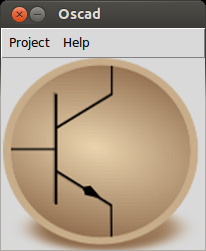
\includegraphics[width=0.5\linewidth]{figures/main-window.png}
\caption{Oscad main window}
\label{main-window}
\end{center}
\end{figure}

Let us open an existing project. Cick on Project and select Open. A window will open asking where is the folder containing the file to be opend. This window is shown in figure\ref{open-directory}. Navigate it to the corresponding directory

\begin{figure}[h]
\begin{center}
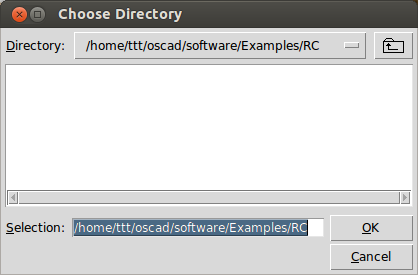
\includegraphics[width=0.5\linewidth]{figures/open-project-directory.png}
\caption{Open project directory}
\label{open-directory}
\end{center}
\end{figure}




